\begin{figure}
  \centering

  \begin{subfigure}[t]{\textwidth}
    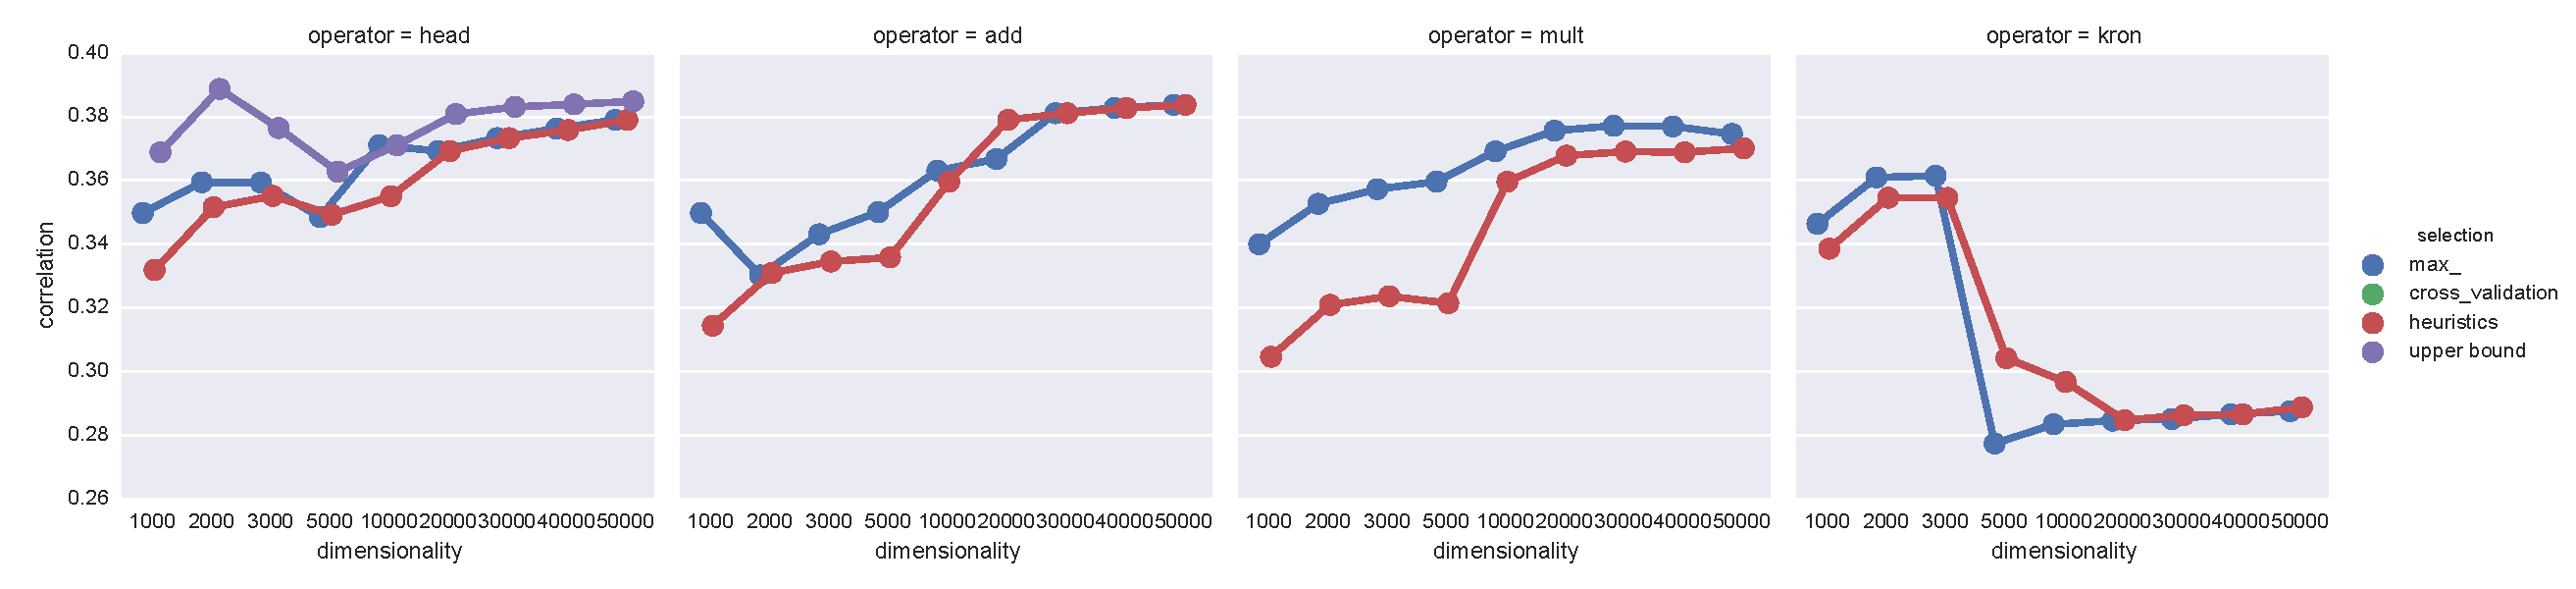
\includegraphics[width=\textwidth]{supplement/figures/universal-results-simlex999}
    \caption{SimLex999}
    \label{fig:universal-results-simlex}
  \end{subfigure}

  \begin{subfigure}[t]{\textwidth}
    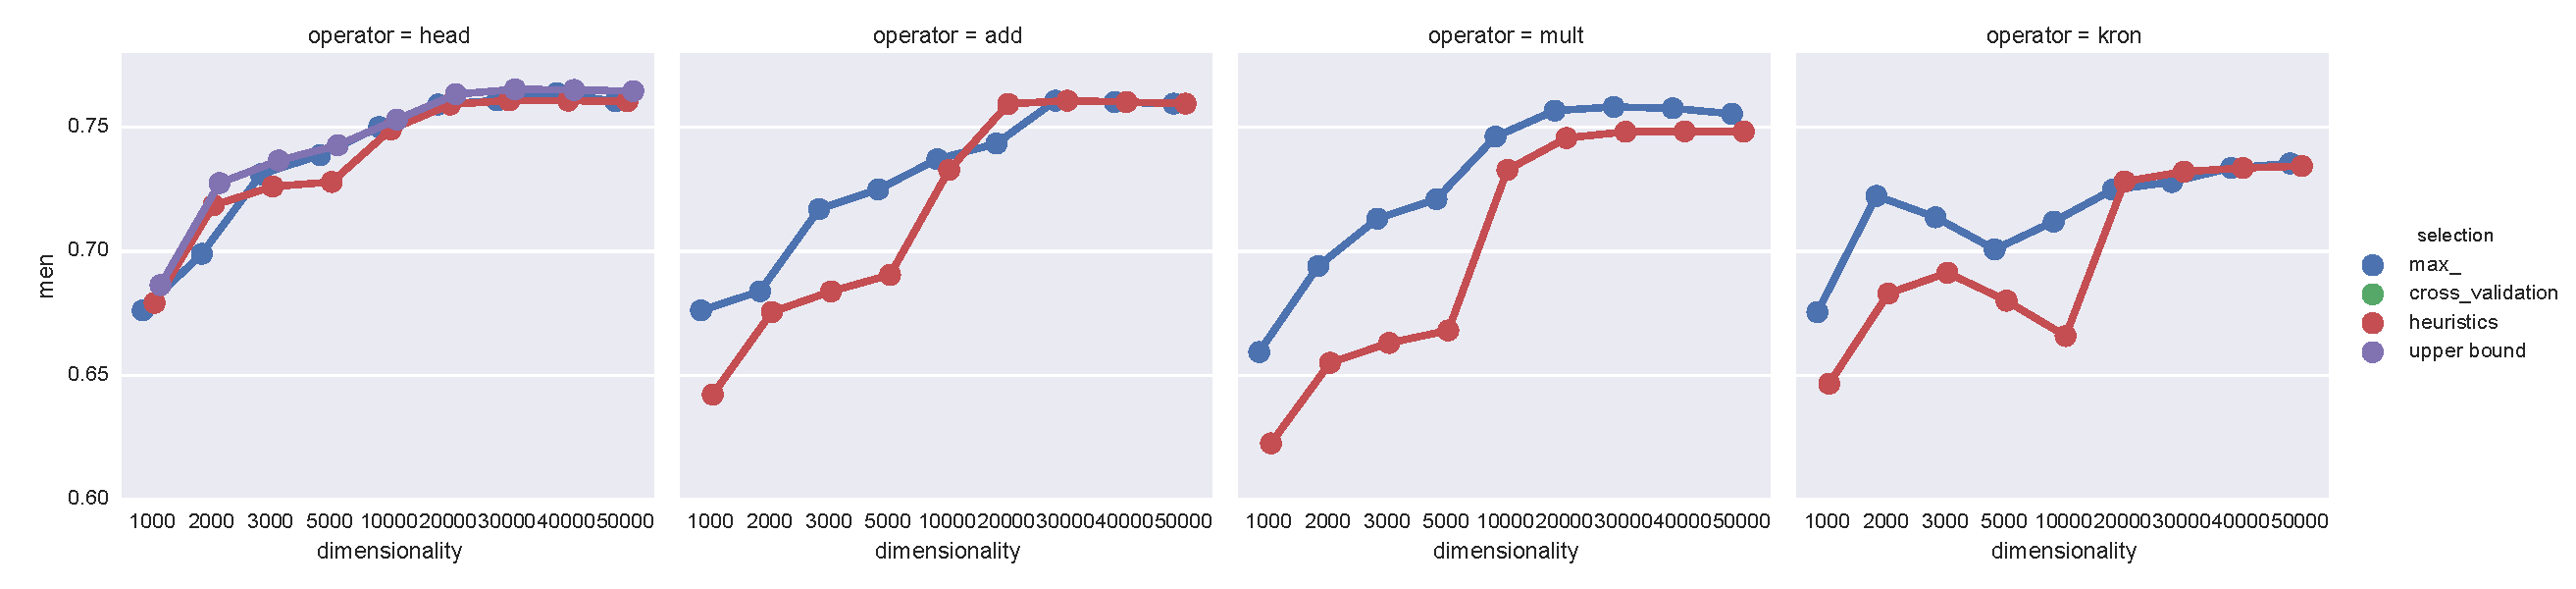
\includegraphics[width=\textwidth]{supplement/figures/universal-results-men}
    \caption{MEN}
    \label{fig:universal-results-men}
  \end{subfigure}


  \begin{subfigure}[t]{\textwidth}
    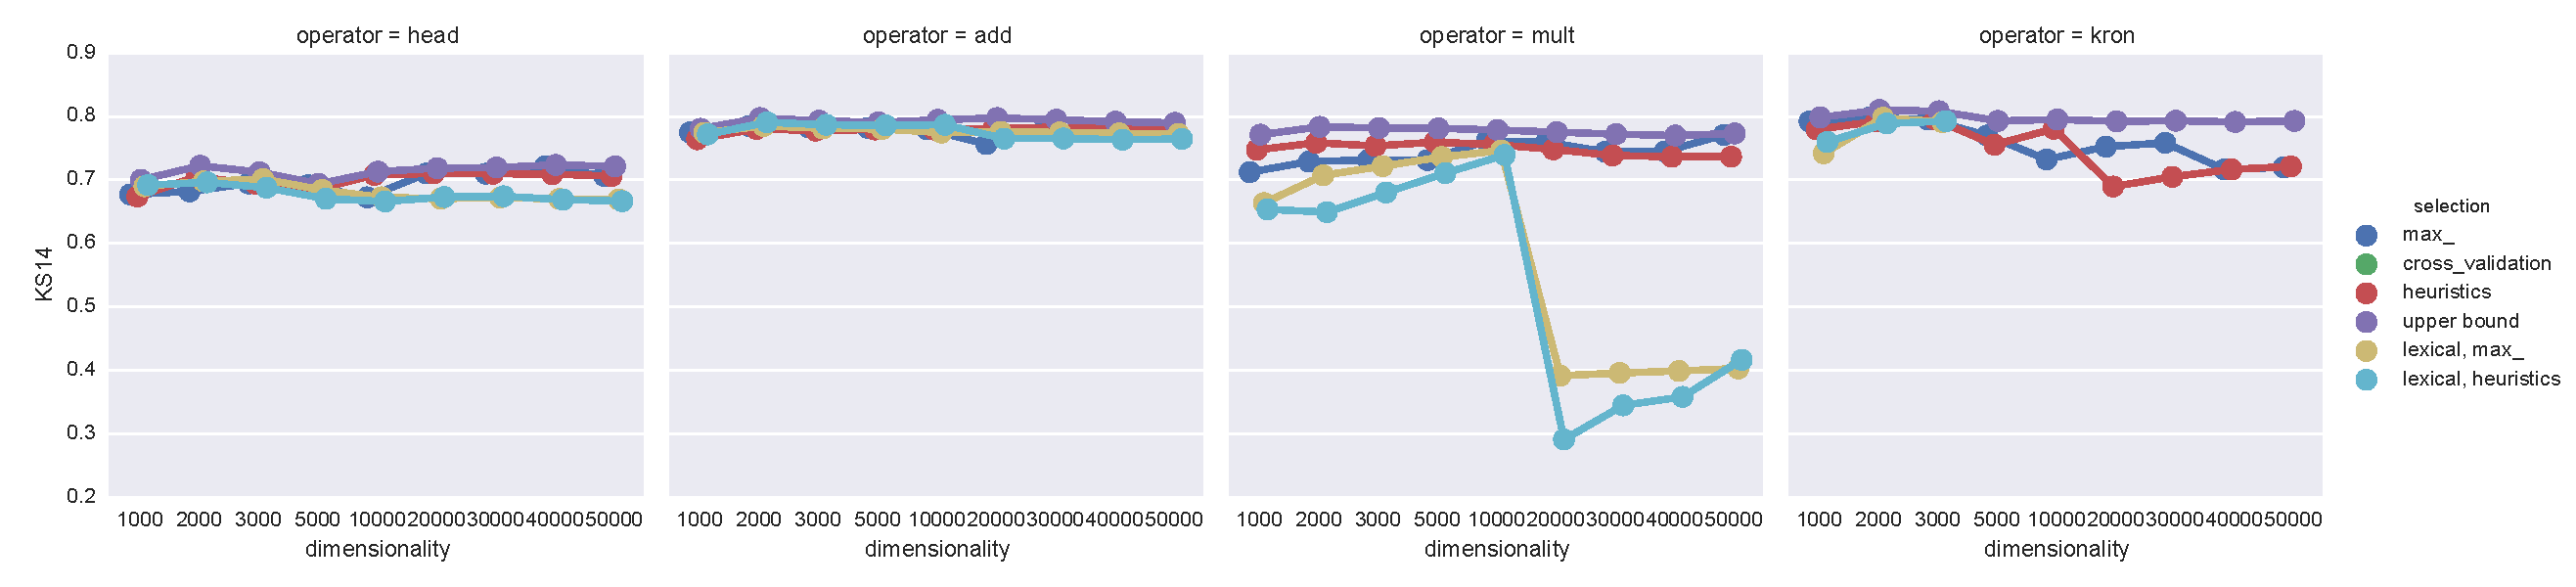
\includegraphics[width=\textwidth]{supplement/figures/universal-results-ks14}
    \caption{KS14}
    \label{fig:universal-results-ks14}
  \end{subfigure}

  \begin{subfigure}[t]{\textwidth}
    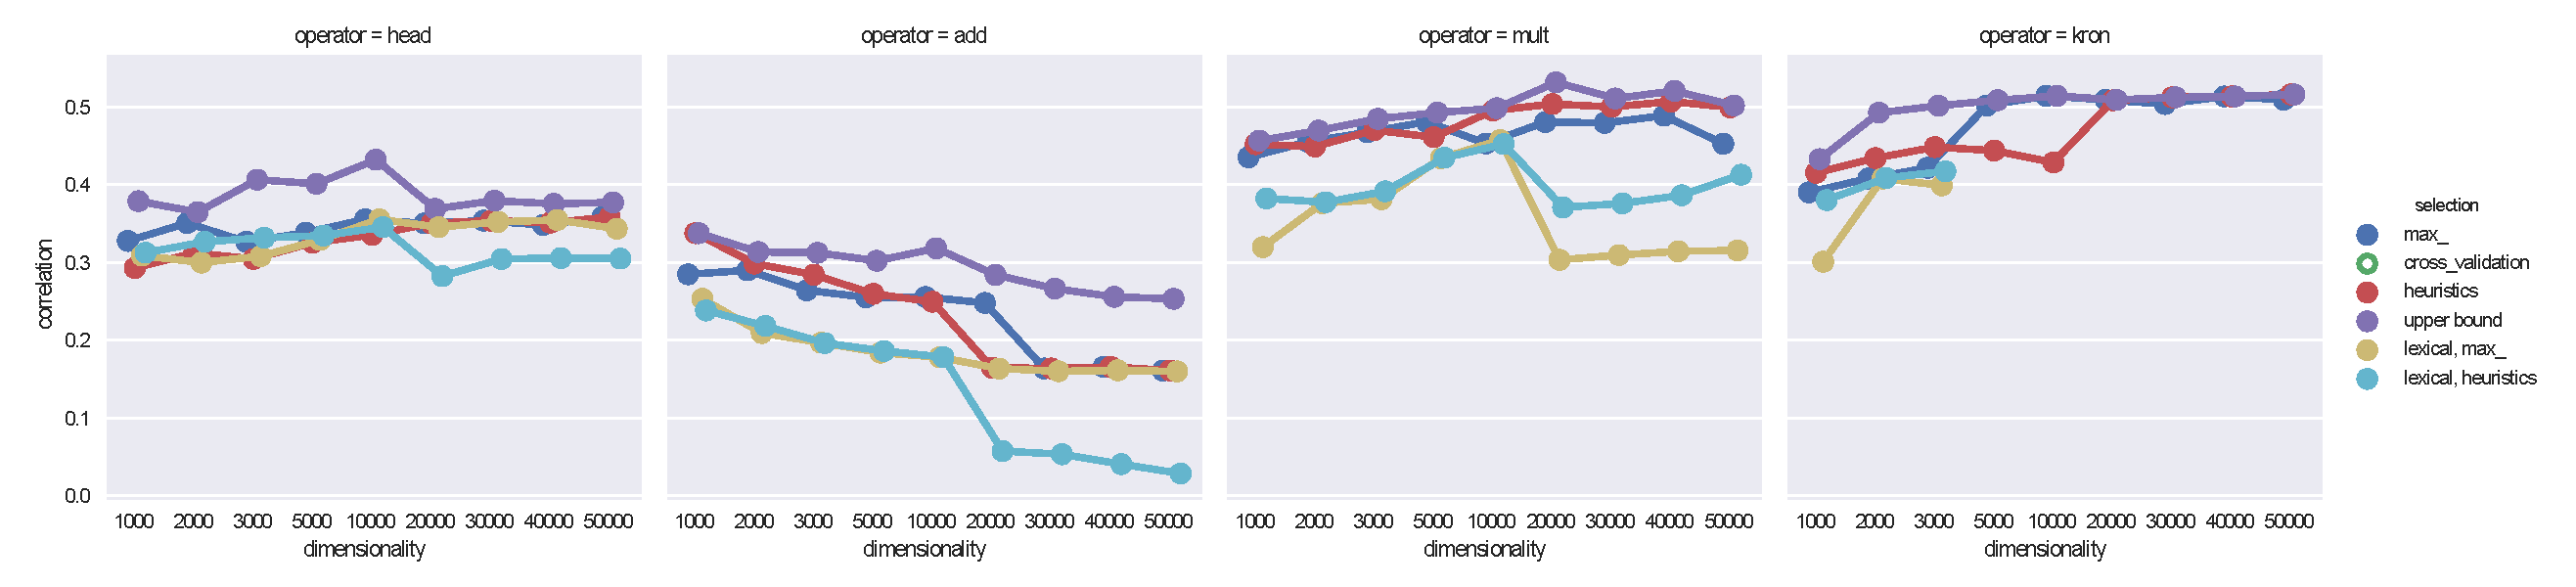
\includegraphics[width=\textwidth]{supplement/figures/universal-results-gs11}
    \caption{GS11}
    \label{fig:universal-results-gs11}
  \end{subfigure}

  \begin{subfigure}[t]{\textwidth}
    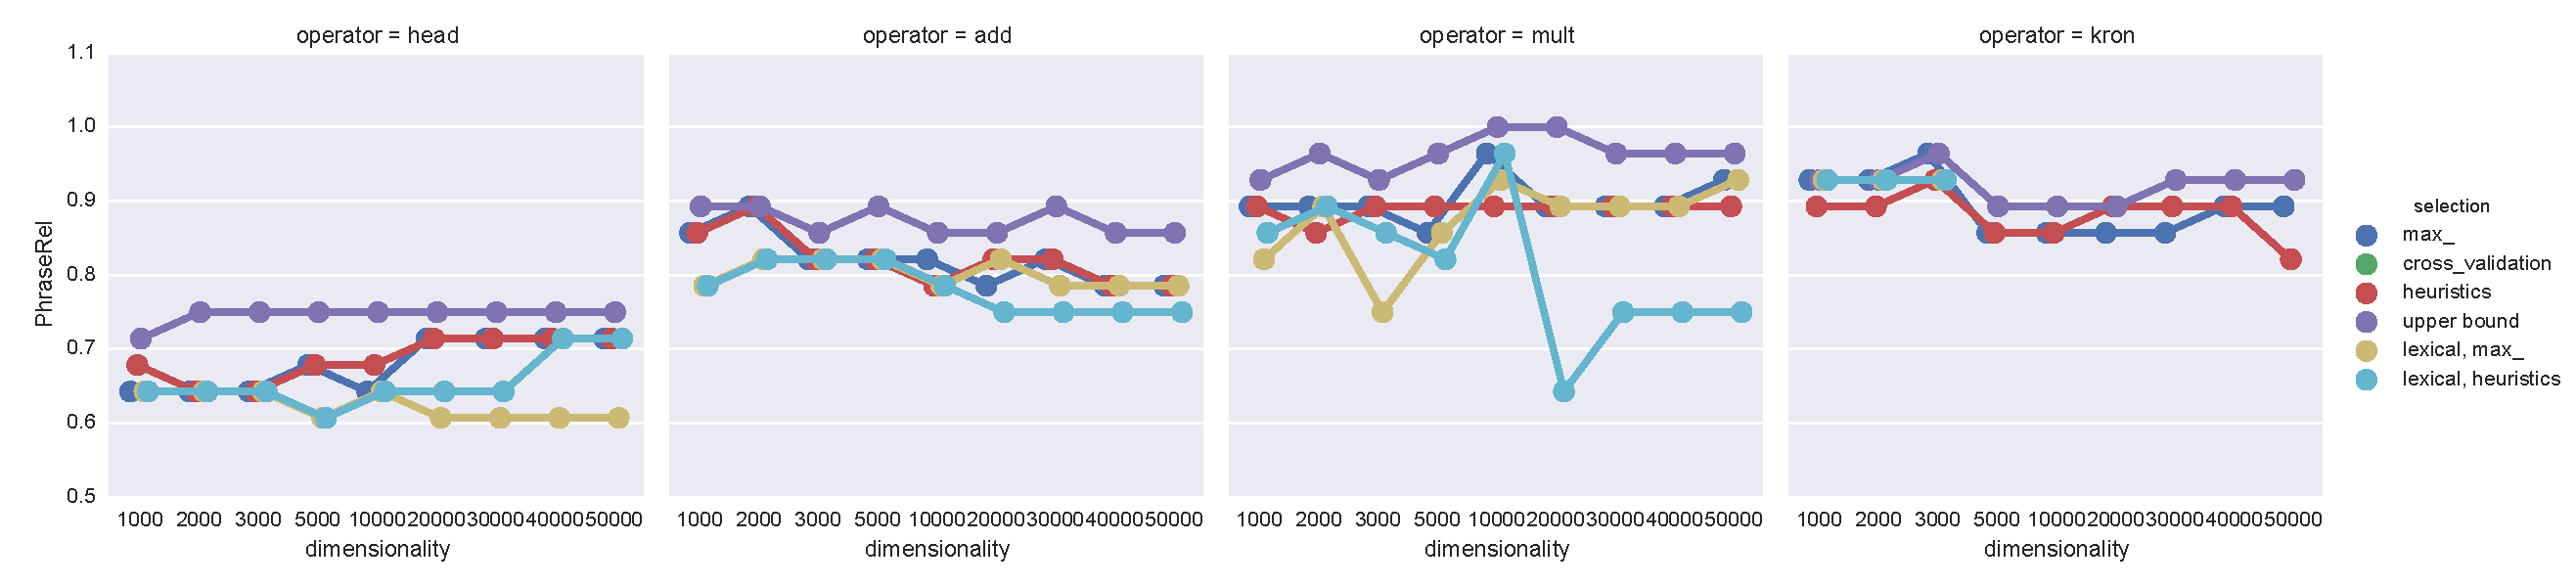
\includegraphics[width=\textwidth]{supplement/figures/universal-results-PhraseRel}
    \caption{PhraseRel}
    \label{fig:universal-results-phraserel}
  \end{subfigure}


  \caption{Performance of models based on the selection over the average universal performance}
  \label{fig:universal-results}
\end{figure}

%%% Local Variables:
%%% mode: latex
%%% TeX-master: "../thesis"
%%% End:
